\chapter{Laboratorio 3}

Il primo circuito analizzato è un rettificatore a doppia semionda di precisione (\Fig\ref{fig:circuito_1}). Grazie all'utilizzo di due amplificatori operazionali ed un diodo, è possibile eliminare i problemi relativi al rettificatore a doppia semionda visto nella precedente esperienza di laboratorio, dove veniva utilizzato un unico amplificatore operazionale e due diodi. Per questo circuito sono stati utilizzati due amplificatori operazionali \textit{general-purpose} \textbf{\textmu A741} \url{https://www.ti.com/lit/ds/symlink/ua741.pdf}.
\begin{figure}[ht!]
	\centering
	\begin{minipage}{.45\textwidth}
		\scalebox{.73}{
			\begin{circuitikz}
				\draw (0,-.5) node[ground]{};
				\draw (0,1) coordinate (vin) to[sV=$v_{in}$] (0,-.5);
				\draw (vin) -- ++(0,1);
				\draw (0,2) -- ++(.32,0) to[R=$R_2$] ++(3,0);
				\draw (3,2) to (4,2);
				\draw (3.7,2) node[op amp, anchor=-](oa){\texttt{\textmu A741}};
				\draw (oa.down) ++(.5,.2) node[below]{$A1$};
				\draw (oa.up) -- ++(0, .3) node[vcc]{$+E$};
				\draw (oa.down) -- ++(0,-.3) node[vee]{$-E$};
				\draw (vin) to[R=$R_1$] (oa.+);
				\draw (1.32,-2) node[op amp, anchor=-](oa2){\texttt{\textmu A741}};
				\draw (oa2.down) ++(.5,.2) node[below]{$A2$};
				\draw (oa.+) -- ++(0,-1) to[D=$D_1$, invert] (oa2.out-|oa.+) to[short, -o] ++(0,0) ++(0,-.1) node[below]{$v_{out2}$};
				\draw (oa2.-) -- ++(0,2) -- ++(2.4,0);
				\draw (oa2.up) -- ++(0, .3) node[vcc]{$+E$};
				\draw (oa2.down) -- ++(0,-.3) node[vee]{$-E$};
				\draw (oa2.+) -- ++(0,-.3) node[ground]{};
				\draw (oa.up) -- ++(0, .3) node[vcc]{$+E$};
				\draw (oa.down) -- ++(0,-.3) node[vee]{$-E$};
				\draw (oa2.+) to[short,-o] ++(0,0) node[left]{$v^2_+$};
				\draw (oa2.-) to[short,-o] ++(0,0) node[left]{$v^2_-$};
				\draw (oa.+) to[short,-o] ++(0,0) node[above]{$v^1_+$};
				\draw (oa.-) to[short,-o] ++(0,0) node[above]{$v^1_-$};
				\draw (3,2) -- ++(0,2) coordinate(C) to[R=$R_3$] ++(3.08,0) (C-|oa.out) coordinate(Co) to[short, -] (oa.out) -- ++(1,0) coordinate(vmin) to [short, -o] ++(1,0) ++(.1,.1) node[above]{$v_{out}$};
				\draw[thick] (-1,-4.5) rectangle (9,5);
			\end{circuitikz} 
		}
	\end{minipage}\qquad
	\begin{minipage}{.45\textwidth}
		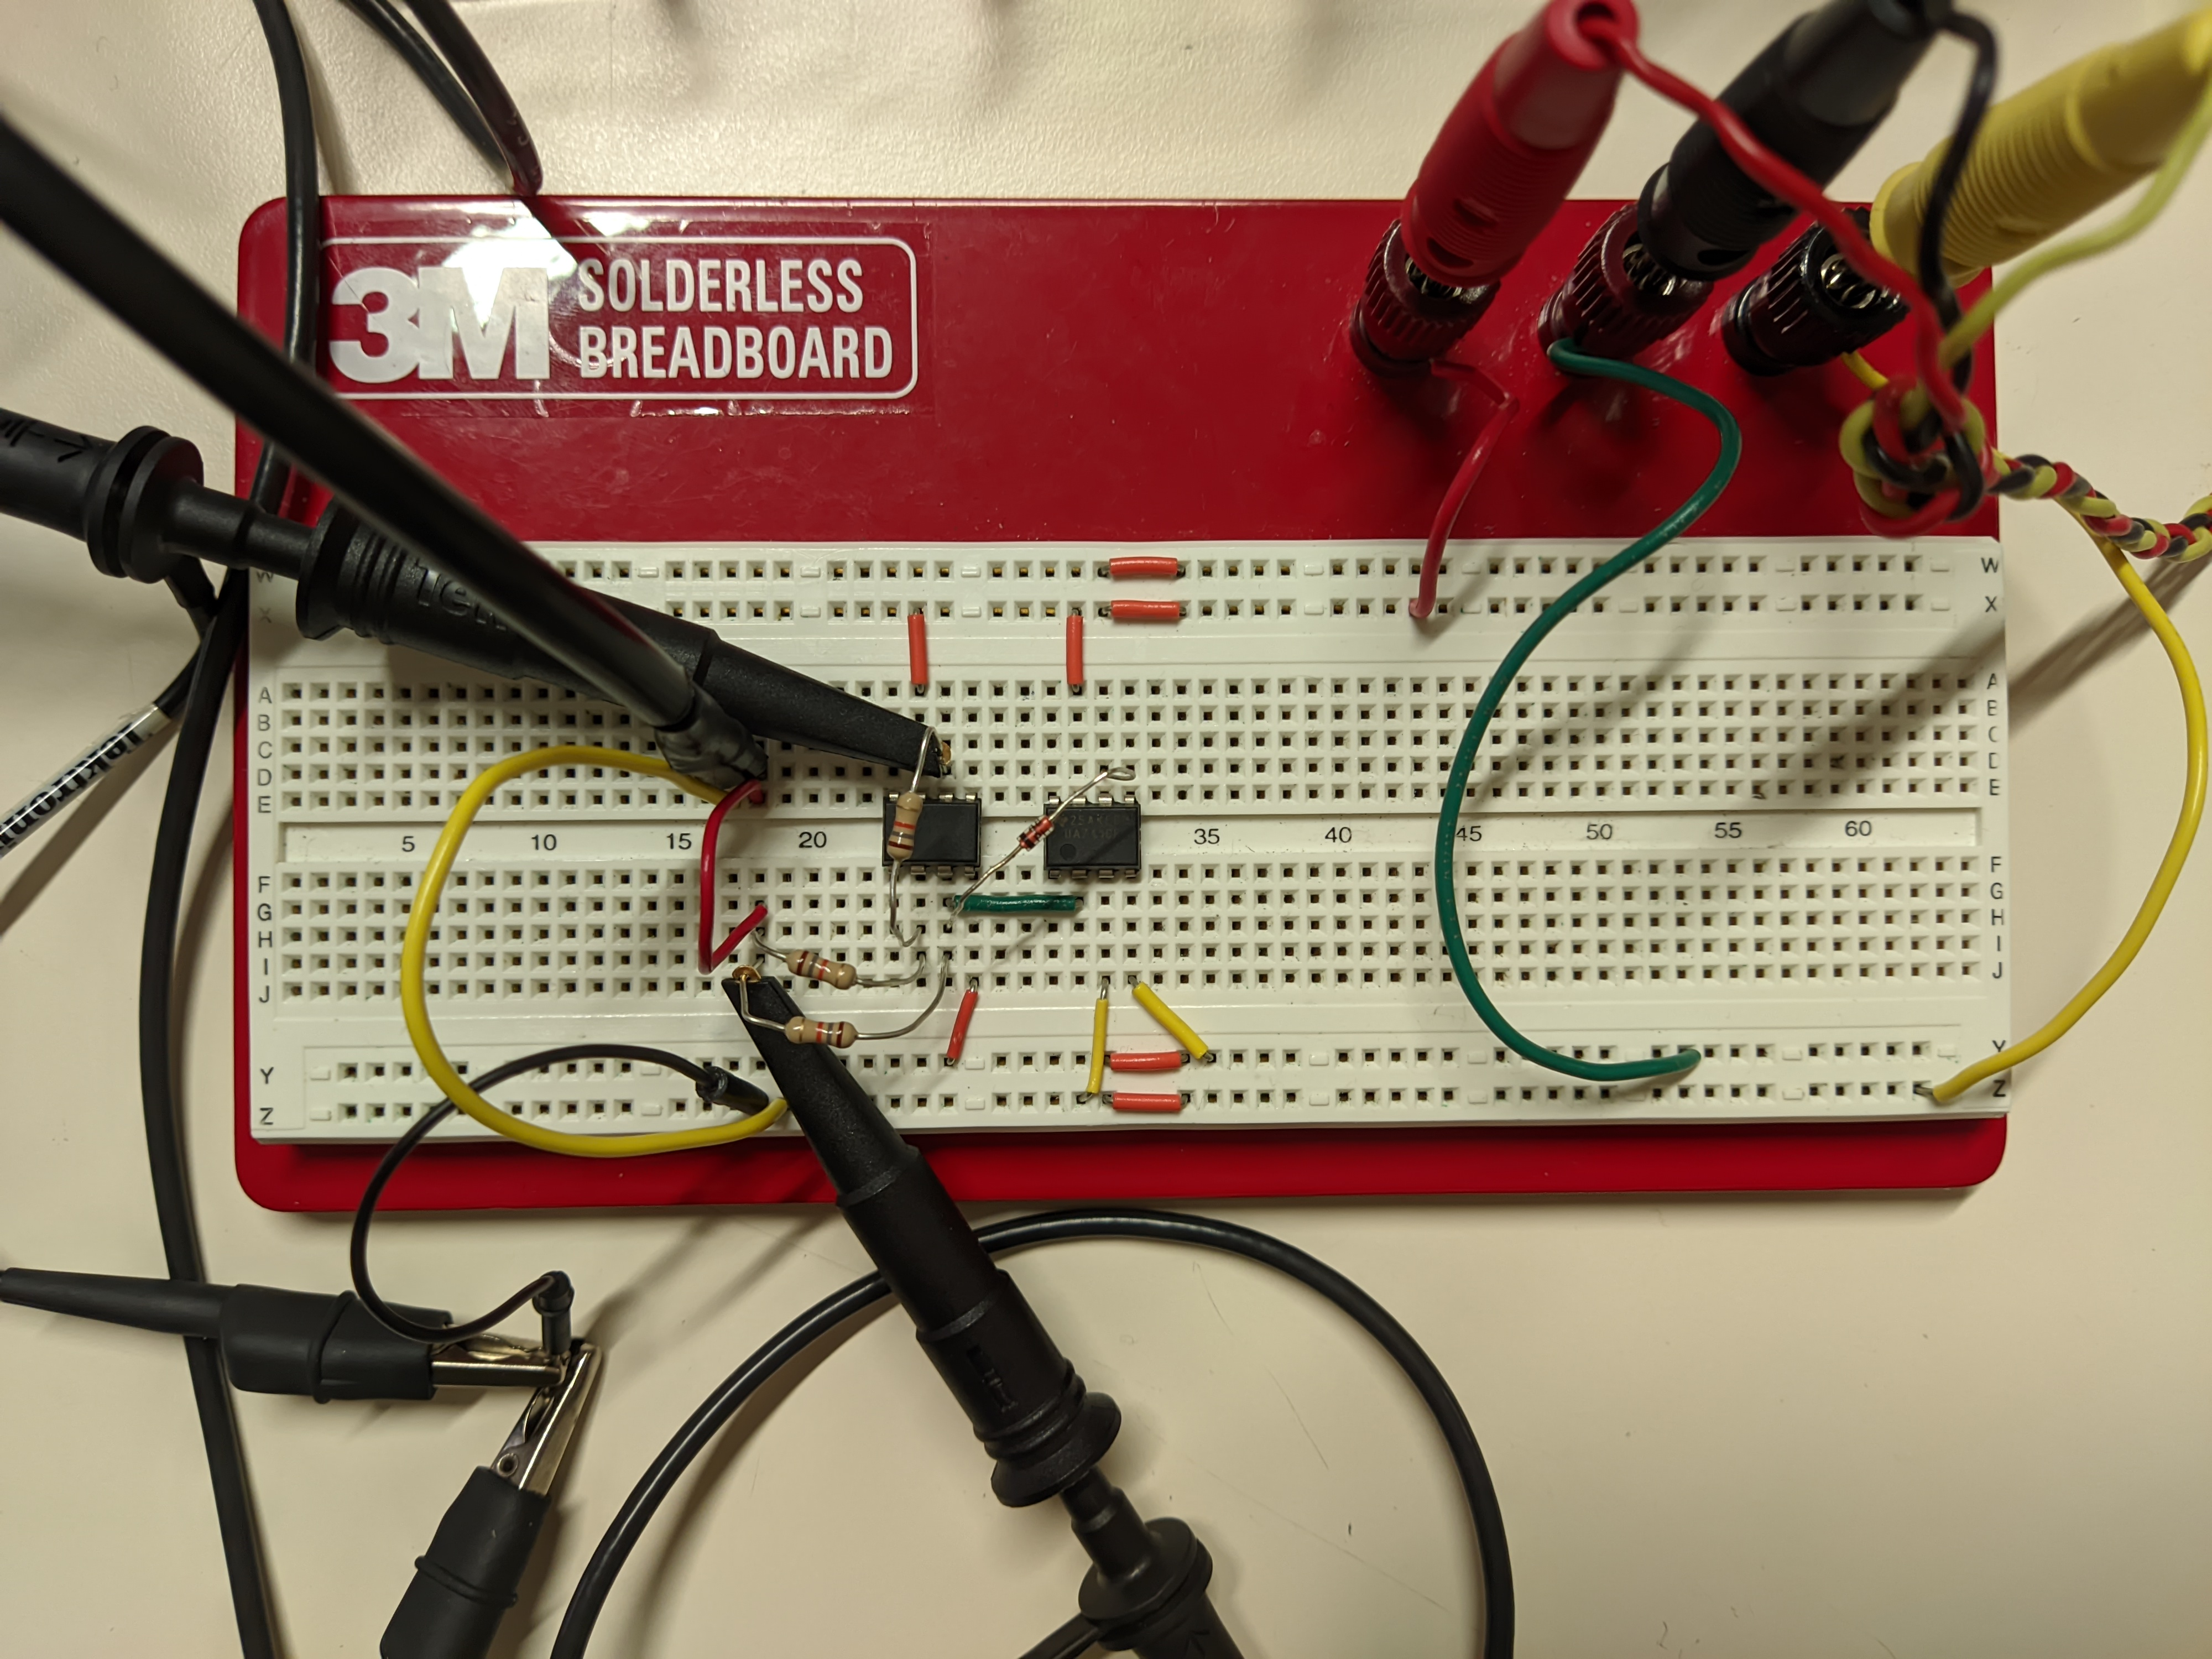
\includegraphics[width=\linewidth]{./ImageFiles/Laboratorio 3/CIR21.jpg}
	\end{minipage}
	\caption{Schema circuitale del raddrizzatore a doppia semionda e foto del circuito realizzato.}
	\label{fig:circuito_1}
\end{figure}

\noindent
Per studiare il comportamento del sistema è necessario analizzare come si comporta il diodo al variare della tensione di ingresso $v_{in}$:
\begin{itemize}
	\item $v_{in} \geq 0$: si ipotizza inizialmente che il diodo sia acceso. Allora, $A2$  è in retroazione negativa. Di conseguenza vale il principio di cortocircuito virtuale e quindi il nodo $v_{+}^1$ è a massa. Se questo fosse vero, la corrente dovrebbe percorrere la resistenza $R1$ da sinistra verso destra\todo{Nominiamo le resistenze anche se hanno lo stesso valore se non spiegare il circuito è un casino. le nominiamo dal basso all'alto, quindi R1 è quella più in basso. Marco: Dovrebbe essere giusto, verificate}. Tuttavia, ciò non è possibile, perchè i morsetti dell'amplificatore operazionale non assorbono corrente e il diodo non permette il passaggio di corrente in quel verso. Quindi, l'ipotesi che il diodo sia acceso non è corretta e assumiamo che il diodo è spento. Questo significa che l'amplificatore $A2$ non è retroazionato. Allora, in $R1$ non può scorrere corrente e la tensione sul nodo $v_{+}^1$ è pari a $v_{in}$. Ma questo implica che anche la tensione sul nodo $v_{-}^1$ sia pari a $v_{in}$. Di conseguenza, non scorre corrente neanche in $R2$ e quindi nemmeno in $R3$. Allora, la tensione $v_{out} = v_{in}$;
	\item $v_{in} < 0$: si ipotizza che il diodo sia acceso, quindi $A2$ è retroazionato negativamente. Il nodo $v_{+}^1$ è connesso ad una massa virtuale e quindi la corrente scorre nella resistenza $R1$ da destra a sinistra, dato che $v_{in} < 0$. Tale corrente può provenire dal diodo e questo verifica l'ipotesi iniziale. Se $v_{+}^1$ è a massa, lo è anche $v_{-}^1$, quindi $A1$ è in configurazione invertente. Se $R2 = R3$, il guadagno dell'amplificatore invertente è pari a 1 e $v_{out} = -v_{in}$.
\end{itemize}
Di conseguenza, questo circuito rettifica entrambe le semionde e elimina il problema dello \text{shift} di tensione causato dalla tensione di polarizzazione del diodo. Nella figura \todo{inserire figura 01} è possibile verificare il comportamento del circuito.

I valori nominali ed effettivi delle resistenze utilizzate e la tensioni di soglia del diodo (misurata tramite multimetro) sono riportati in tabella \ref{xxx}.

\todo{inserire tabella con valori effettivi e misurati anche del diodo come nelle scorse relazioni e aggiungere indicazioni tensione +E e -E}

\noindent
Inoltre, si può verificare la caratteristica ingresso-uscita del circuito analizzando il grafico XY generato dall'oscilloscopio \todo{inserire figura 00}. Questo grafico mostra la tensione di uscita (asse delle ordinate) in funzione della tensione in ingresso (asse delle ascisse) e rappresenta una funzione di valore assoluto: infatti, il compito di un rettificatore è quello di riportare inalterato il segnale in ingresso in uscita, se positivo, ed invertirlo se negativo.

\noindent
Successivamente, si è analizzato il comportamento in frequenza del circuito effettuando delle misure di $v_{in}$ e $v_{out}$ con l'oscilloscopio, variando la frequenza della sinusoide in ingresso. \todo{inserire foto 01,03,04,05}
\`E possibile notare che dalla frequenza di \SI{1}{\kilo\hertz} l'uscita presenta un ritardo sul fronte di salita ed a partire dai \SI{10}{\kilo\hertz} il circuito non funziona più come un raddrizzatore. Questo comportamento è legato allo \textit{slew rate} dell'amplificatore \textit{A2}: infatti, quando il diodo è spento, \textit{A2} non è più in retroazione e l'uscita $v_{out}^2$ satura alla tensione di saturazione negativa (poiché $v_+^2$ è a massa e $v_-^2=v_{in}>0$).\todo{aggiungere immagine 02} Il nodo $v_{out}^2$ dovrebbe quindi passare dalla tensione -E a \SI{0}{\volt} con una pendenza pari ad infinito, ma ciò è impossibile. Dal datasheet si ricava che lo \textit{slew rate} del \textbf{\textmu A741} è pari a \SI{0.5}{\volt\per\micro\second}. Si è cercato di stimare questo parametro delle misure effettuate \todo{inserire figura 06}. Il valore stimato è di circa $\frac{\SI{8.11}{\volt}}{\SI{20.0}{\micro\second}}=\SI{0.41}{\volt\per\micro\second}$, compatibile con le indicazioni presenti sul datasheet.

\clearpage
Il secondo circuito analizzato è chiamato \textit{Trigger di Schmitt} e svolge la funzione di comparatore con isteresi (\Fig\ref{circuito_2}). 
\begin{figure}[h!]
	\centering
	\begin{minipage}{.45\textwidth}
	\end{minipage}\qquad
	\begin{minipage}{.45\textwidth}
		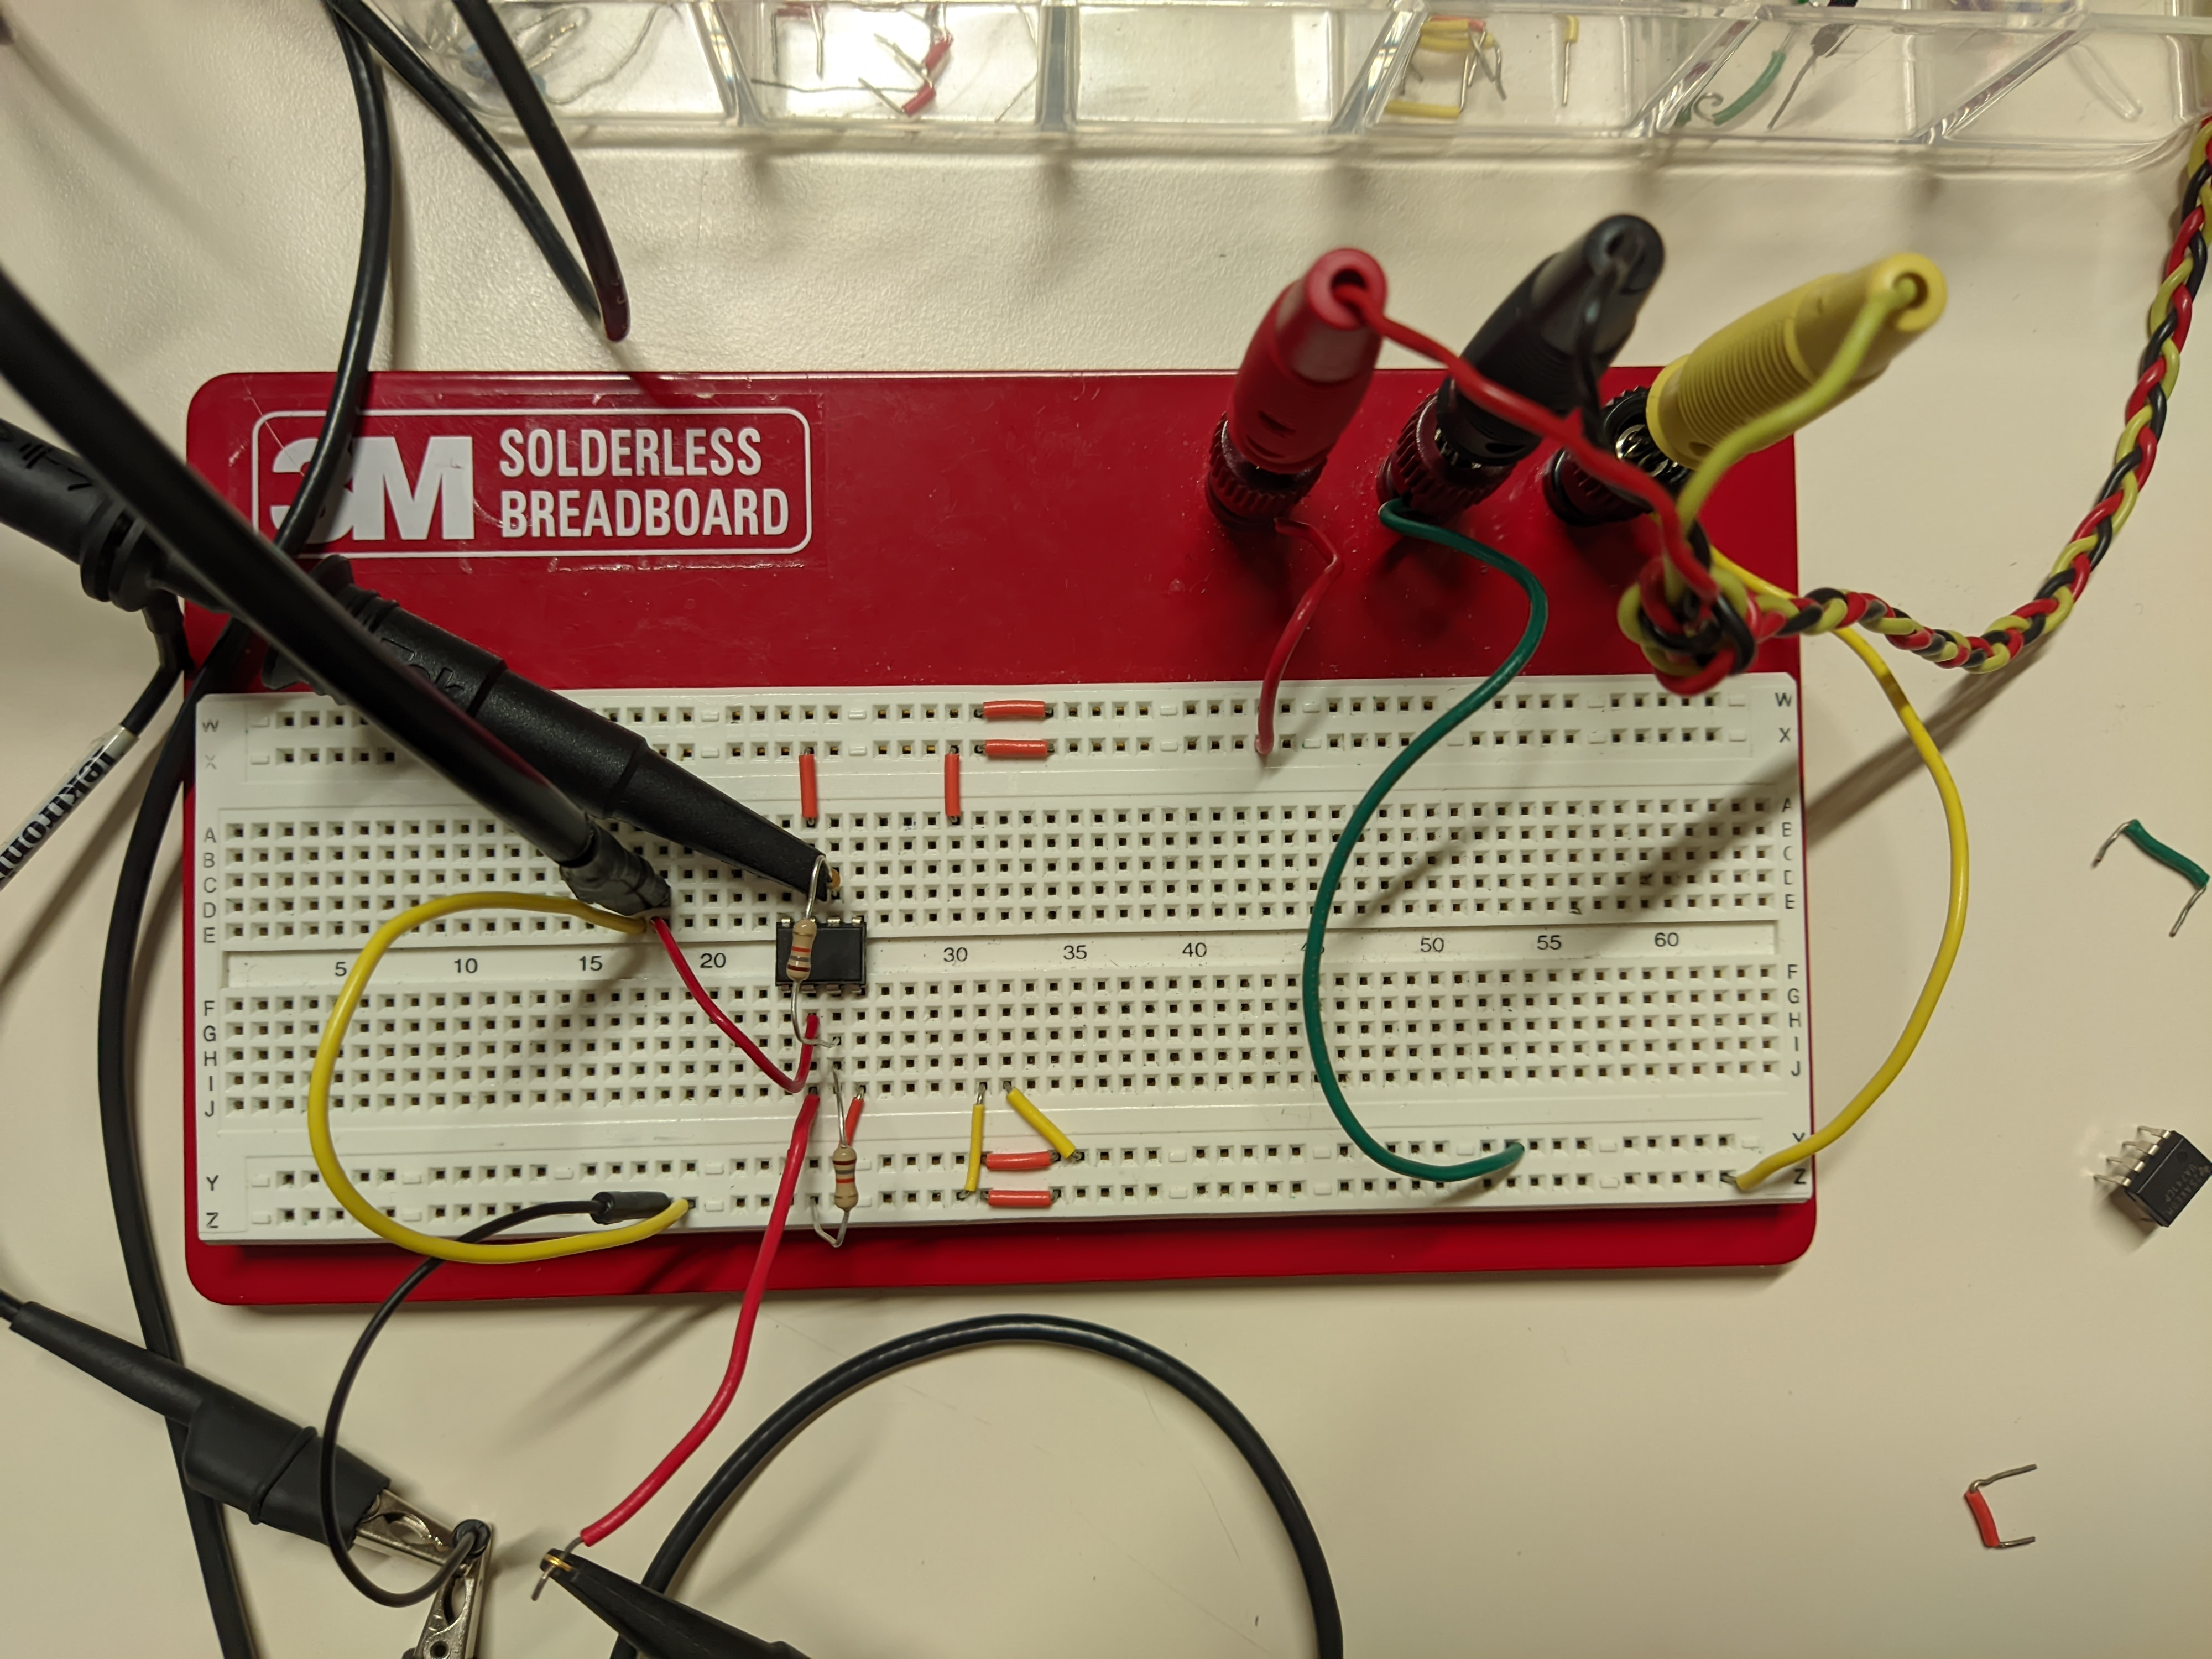
\includegraphics[width=\linewidth]{./ImageFiles/Laboratorio 3/CIR12.jpg}
	\end{minipage}
	\caption{Schema circuitale del \textit{Trigger di Schmitt} e foto del circuito realizzato.}
	\label{fig:circuito_2}
\end{figure}

Come si può osservare nel circuito, il segnale di ingresso $v_{in}$ viene applicato al morsetto invertente di un amplificatore operazionale (nel nostro caso si è utilizzato il \textbf{\textmu A741}), retroazionato positivamente grazie alle resistenze $R\sub{1}$ e $R\sub{2}$. Di conseguenza, non è più valido il principio di cortocircuito virtuale tra $V\super{+}$ e $V\super{-}$, poiché non è più presente una retroazione negativa. Per cui, l'uscita $v_{out}=A(v^+-v^-)$, con A pari al guadagno dell'amplificatore operazionale, e il circuito si comporta come un comparatore. Infatti, supponendo un guadagno molto alto (idealmente tendente all'infinito), accade che:
\begin{itemize}
	\item se $v^+-v^->0$, allora $v_{out}=+E$;
	\item se $v^+-v^-<0$, allora $v_{out}=-E$.
\end{itemize}
Tuttavia, nel \textit{Trigger di Schmitt} la soglia alla quale l'uscita passa dalla tensione di saturazione positiva a quella negativa è diversa rispetto a quella vista prima di un normale comparatore. Le resistenze $R\sub{1}$ e $R\sub{2}$ definiscono un partitore di tensione per cui $v^+=\frac{R_1}{R_1+R_2}v_{out}$. Supponendo che inizialmente la tensione $v_{in}$ sia pari a -E, di conseguenza l'uscita $v_{out}$ saturerà alla tensione +E (in quanto $v_{in}$ è applicata al morsetto invertente). Infatti, la tensione al nodo $v^+$ sarà pari a $v^+=\frac{R_1}{R_1+R_2}(+E)=V_H^+$ e se $R_1=R_2$ risulta che $V_H^+=\frac{1}{2}(+E)$. Per cui, fintanto che la tensione $v_{in}$ sarà minore della tensione $V_H^+$, l'uscita resterà alla tensione +E. Quando si avrà che $v_{in}>V_H^+$, l'uscita si porterà alla tensione di saturazione negativa -E e rimarrà tale fino a quando $v_{in}<V_L^+=\frac{R_1}{R_1+R_2}(-E)\overset{\mathrm{R_1=R_2}}{=}V_L^+=\frac{1}{2}(-E)$. 

\noindent
Riassumendo, in uscita si avrà un'onda quadra che commuta tra la tensione +E e -E, con \textit{duty-cycle} regolato dal periodo del segnale in ingresso. \todo{Verificare bene questa frase, mi sembra che possa essere fraintesa.}

\todo{magari inserire un grafico fatto tipo a mano su onenote per esempio delle soglie che magari è più pratico?}

I valori nominali ed effettivi delle resistenze utilizzate sono riportati in tabella \ref{tab:valori_componenti_2}.

\def\arraystretch{1.3}
\begin{table}[h]
	\centering
	\begin{tabular}{|c|c|c|}
		\hline
		Componente	& Valore Nominale & Valore Misurato \\ \hline
		R1 & & \\ \hline
		R2 & & \\ \hline
	\end{tabular}
	\caption{Valori nominali e misurati delle resistenze utilizzate nel circuito.}
	\label{tab:valori_componenti_2}
\end{table}

\todo{continuare spiegazione }

\todo{inserire valori resistenze reale}
L'utilizzo di questa struttura è molto utile perché è meno sensibile rispetto ai disturbi che possono esserci sul segnale in ingresso al sistema. Infatti, se il segnale in ingresso fosse molto disturbato, con un comparatore classico in corrispondenza della soglia l'uscita continuerebbe ad oscillare fino a che il segnale in ingresso con il disturbo sommato non supera abbondantemente la soglia. In un comparatore con isteresi questo problema non si pone: infatti, non appena il segnale sommato al disturbo supera la prima soglia, essa cambia ed è necessario che il segnale superi la seconda (\Fig\ref{fig:trigger_di_shmitt_vantaggi}).

\begin{figure}[h!]
	\centering
	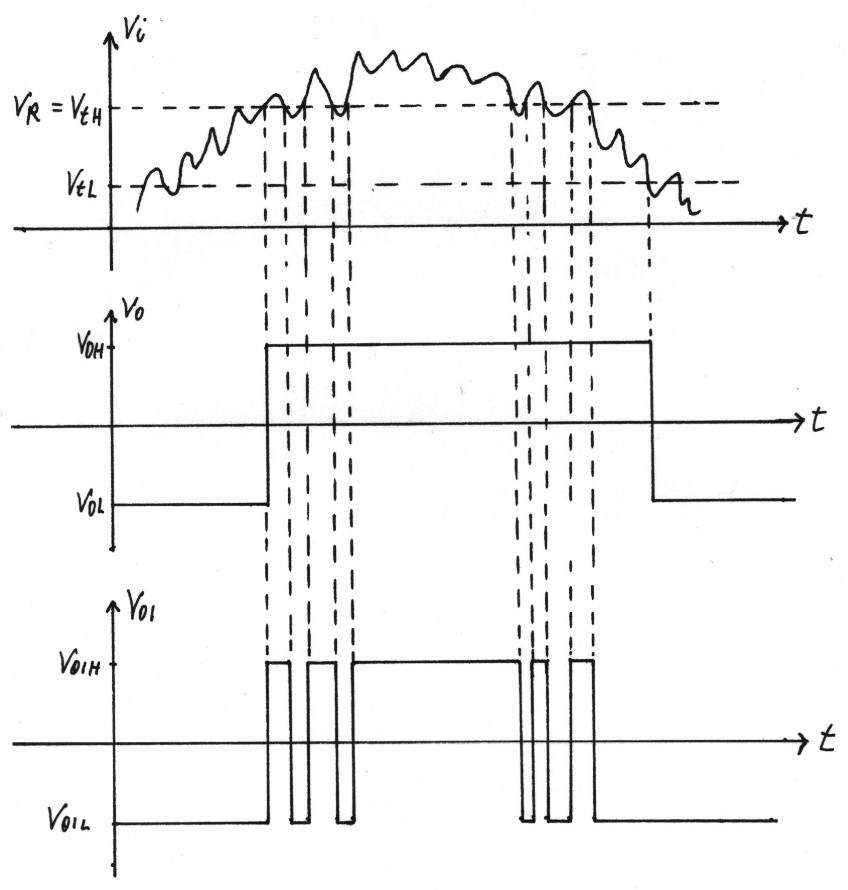
\includegraphics[width=\linewidth]{./ImageFiles/Laboratorio 3/Usicta Rumorosa e Trigger di Shmitt.jpg}
	\caption{In questi grafici viene confrontato il comportmento di un comparatore classico (grafico in basso) con uno a \textit{Trigger di Schmitt} (grafico in mezzo) quando il segnale in ingresso è rumoroso (grafico in alto).}
	\label{fig:trigger_di_shmitt_vantaggi}
\end{figure} 

La caratteristica ingresso-uscita di un comparatore a \textit{Trigger di Schmitt} è un ciclo di isteresi (\Fig\ref{fig:ciclo_isteresi}): come si può vedere dal grafico, in funzione al verso di percorrenza, le tensioni di soglia sono differenti. 
\begin{figure}[h!]
	\centering
	\includegraphics[width=\linewidth]{./ImageFiles/Laboratorio 3/Ciclo di Isteresi.png}
	\caption{Ciclo di isteresi del \textit{Trigger di Schmitt}.}
	\label{fig:ciclo_isteresi}
\end{figure} 
\todo{inserire caratteristica ingresso uscita con anche la foto oscilloscopio}


\clearpage
Il terzo circuito analizzato è un oscillatore (\Fig\ref{fig:circuito_3}). Un circuito oscillatore produce in uscita un'onda quadra, senza che in ingresso vi sia applicato un segnale.

 \begin{figure}[h!]
 	\centering
 	\begin{minipage}{.45\textwidth}
 	
 	\end{minipage}\qquad
 	\begin{minipage}{.45\textwidth}
 		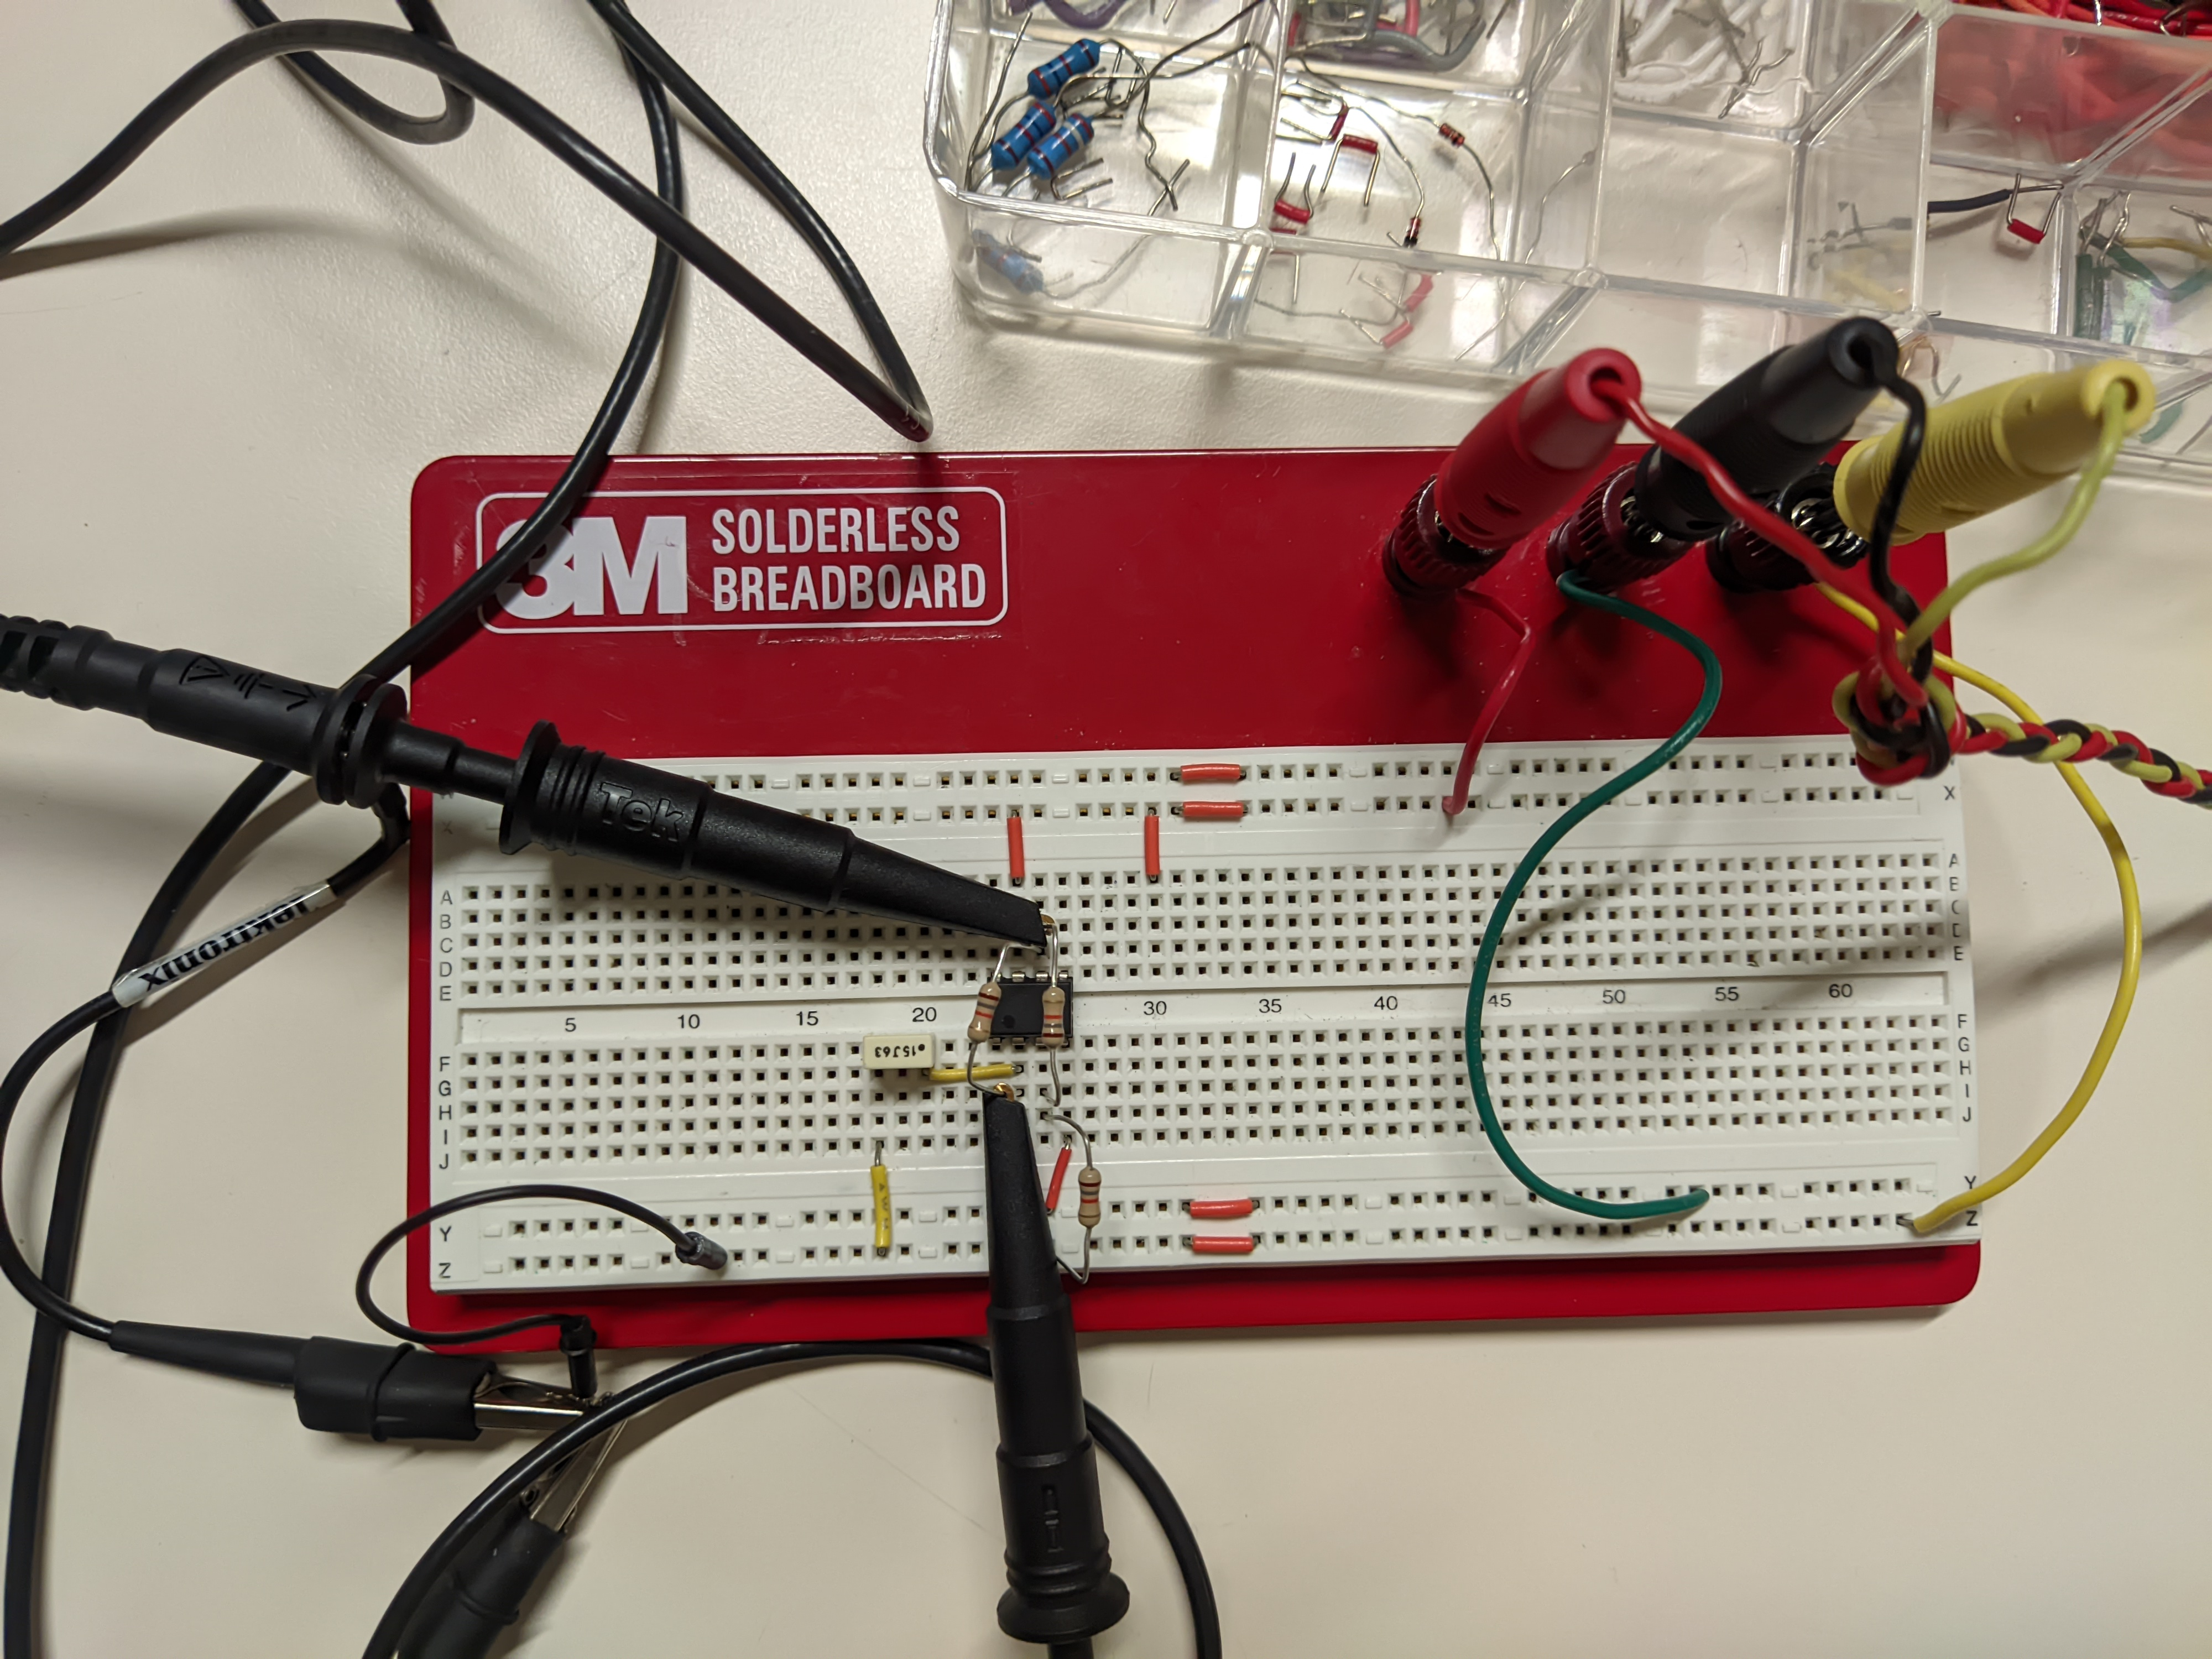
\includegraphics[width=\linewidth]{./ImageFiles/Laboratorio 3/CIR31.jpg}
 	\end{minipage}
 	\caption{Schema circuitale dell'oscillatore e foto del circuito realizzato.}
 	\label{fig:circuito_3}
 \end{figure}

Per valutare il comportamento del circuito è necessario fare le seguenti osservazioni:
\begin{itemize}
	\item l'amplificatore è retroazionato positivamente, per cui l'uscita commuta tra $V_{DD}$ e $V_{SS}$;
	\item la tensione di soglia dipende in modo dinamico dalla tensione di uscita. 
\end{itemize}
Si ipotizzi che la tensione $v^+$ sia maggiore della tensione $v^-$, per cui l'uscita $v_{out} = V_{DD}$ (o una tensione che approssima $V_{DD}$). Allora:
\begin{equation}
	v^+ = \frac{R1}{R1+R2}V_{DD} = V_H^+
\end{equation}
per cui se $R1 = R2$, allora $V_H^+ = V_{DD}/2$. Nell'altra porzione di circuito è presenta una capacità $C$ con in serie la resistenza $R3$. Si ipotizzi che il condensatore sia inizialmente scarico e quindi $V_C = 0$. Se $v_{OUT} = V_{DD}$ allora il condensatore inizia a caricarsi tramite $R3$. Di conseguenza, la tensione al nodo $v_-$ (che è uguale a quella ai capi di $C$) inizia ad aumentare fino a che supera il livello di soglia $V_H^+$. A questo punto, $v^- > v^+$ e quindi $v_{OUT} = V_{SS}$: la tensione ai capi del condensatore è maggiore della tensione in uscita, quindi il condensatore si scarica attraverso $R3$. Ad un certo punto, il condensatore raggiungerà un'altra tensione di soglia pari a:
\begin{equation}
	V_L^+ = \frac{R1}{R1+R2}V_{SS}
\end{equation}
per cui se $R1 = R2$, allora $V_L^+ = V_{SS}/2$. Di conseguenza, $v_{OUT}$ ritorna a $V_{DD}$ e il condensatore comincia nuovamente una fase di carica. Questo ciclo si ripete all'infinito e tale comportamento si può osservare in figura \ref{fig:oscillatore}.

\begin{figure}[h!]
	\centering
	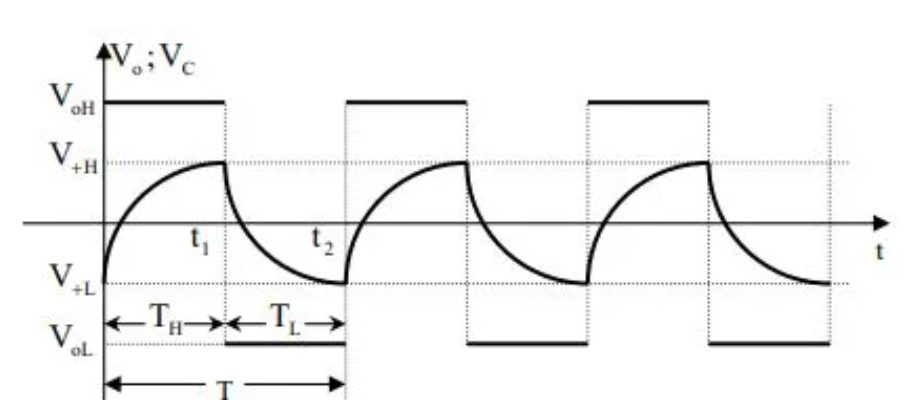
\includegraphics[width=\linewidth]{./ImageFiles/Laboratorio 3/Oscillatore.jpg}
	\caption{Segnali $V_{OUT}$ e $V_C$ in funzione del tempo.}
	\label{fig:oscillatore}
\end{figure} 

La frequenza di oscillazione può essere regolata variando i componenti. In particolare, tale frequenza dipende dalla fase di carica e scarica del condensatore. 
\todo{continuare ocn le formule} 
